\documentclass[11pt]{article}

% Use Helvetica font.
%\usepackage{helvet}
\usepackage{float}


%\usepackage[T1]{fontenc}
%\usepackage[sc]{mathpazo}
\usepackage{color}
\usepackage{amsmath,amsthm,amssymb,multirow,paralist}
\usepackage{graphicx}
%\renewcommand{\familydefault}{\sfdefault}

% Use 1/2-inch margins.
\usepackage[margin=0.8in]{geometry}
\usepackage{hyperref}

\begin{document}

\begin{center}
{\Large \textbf{COM S 4740/5740: Introduction to Machine Learning}

Homework \#1}\\

\linethickness{1mm}\line(1,0){498}

\begin{enumerate}
\item Please put required code files or report into a
compressed file ``HW\#\_FirstName\_LastName.zip''
\item Unlimited number of submissions are
allowed on Canvas and the latest one will be graded.
\item {\color{red} No later submission is accepted.}
\item Please read and follow submission instructions. No exception
will be made to accommodate incorrectly submitted files/reports.
\item All students are required to typeset their reports using
latex. Overleaf
(\url{https://www.overleaf.com/learn/latex/Tutorials}) can be a
good start.
\end{enumerate}

\linethickness{1mm}\line(1,0){498}

\end{center}

%%%%%%%%%%%%%%%%%%%%%%%%%%%%%%%%%%%%%%%%%%%%%%%%%%%%%%%%%%%%%%%%%%%%%%%%%%%%%%%

%%%%%%%%%%%%%%%%%%%%%%%%%%%%%%%%%%%%%%%%%%%%%%%%%%%%%%%%%%%%%%%%%%%%%%%%%%%%%%%


\begin{enumerate}
\item (10 points) Consider the perceptron in two dimensions:
$h(\boldsymbol x) = \mbox{sign}(\boldsymbol w^T \boldsymbol x)$
where $\boldsymbol w = [w_0, w_1, w_2]^T$ and
$\boldsymbol x = [1, x_1, x_2]^T$. Technically, $\boldsymbol x$ has
three coordinates, but we call this perceptron two-dimensional
because the first coordinate is fixed at 1.

\begin{enumerate}

\item Show that the regions on the plane where
$h(\boldsymbol x) = +1$ and $h(\boldsymbol x) = -1$ are separated by
a line. If we express this line by the equation $x_2 = ax_1 + b$,
what are the slope $a$ and intercept $b$ in terms of $w_0, w_1, w_2$?

{\color{red}
\[
h(\boldsymbol{x}) = \text{sign}(\boldsymbol{w}^T \boldsymbol{x})
= \text{sign}(w_0 + w_1 x_1 + w_2 x_2).
\]

decision boundary:
\[
w_0 + w_1 x_1 + w_2 x_2 = 0.
\]

solving for $x_2$:
\[
x_2 = -\frac{w_1}{w_2}x_1 - \frac{w_0}{w_2}.
\]

a and b:
\[
a = -\frac{w_1}{w_2}, \qquad b = -\frac{w_0}{w_2}.
\]
}

\item Draw pictures for the cases $\boldsymbol w = [1,2,3]^T$ and
$\boldsymbol w = -[1,2,3]^T$. Label the positive and negative
prediction regions on the pictures.

{\color{red}

$\boldsymbol{w} = [1,2,3]^T$ 
\\
decision boundary:
\[
1 + 2x_1 + 3x_2 = 0,
\]
\[
x_2 = -\frac{2}{3}x_1 - \frac{1}{3}.
\]

plugging in the origin (0,0):
\[
1 + 2(0) + 3(0) = 1 > 0.
\]
This means the the region containing the origin is positive. 

\begin{figure}[H]
    \centering
    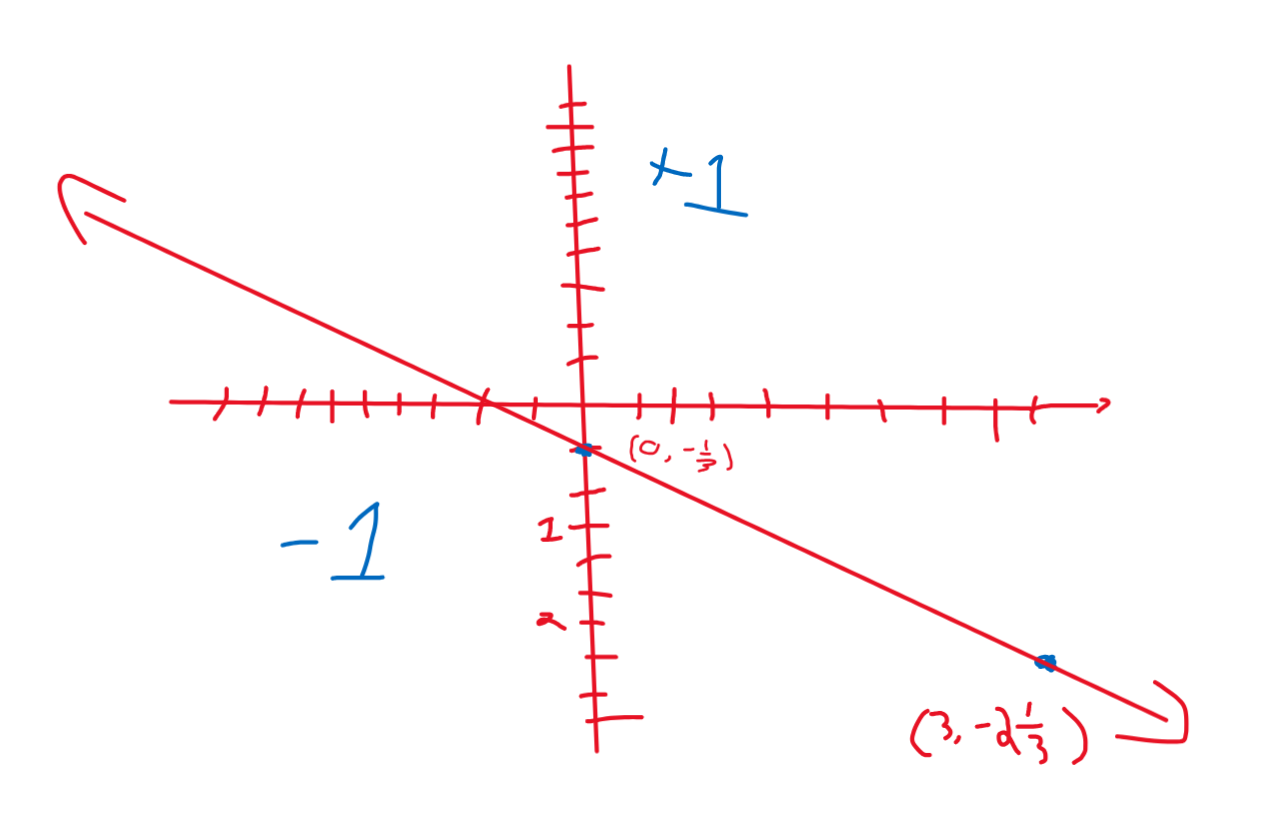
\includegraphics[width=0.6\textwidth]{posneg.png}
    \caption{Decision boundary and classification regions for $\boldsymbol{w} = [1,2,3]^T$.}
    \label{fig:case1}
\end{figure}

$\boldsymbol{w} = -[1,2,3]^T = [-1,-2,-3]^T$.

The decision boundary is
\[
-1 - 2x_1 - 3x_2 = 0,
\]
which represents the same line as before.

plugging in the origin 
\[
-1 - 2(0) - 3(0) = -1 < 0.
\]
this means that the region with the origin is the negative region now

\begin{figure}[H]
    \centering
    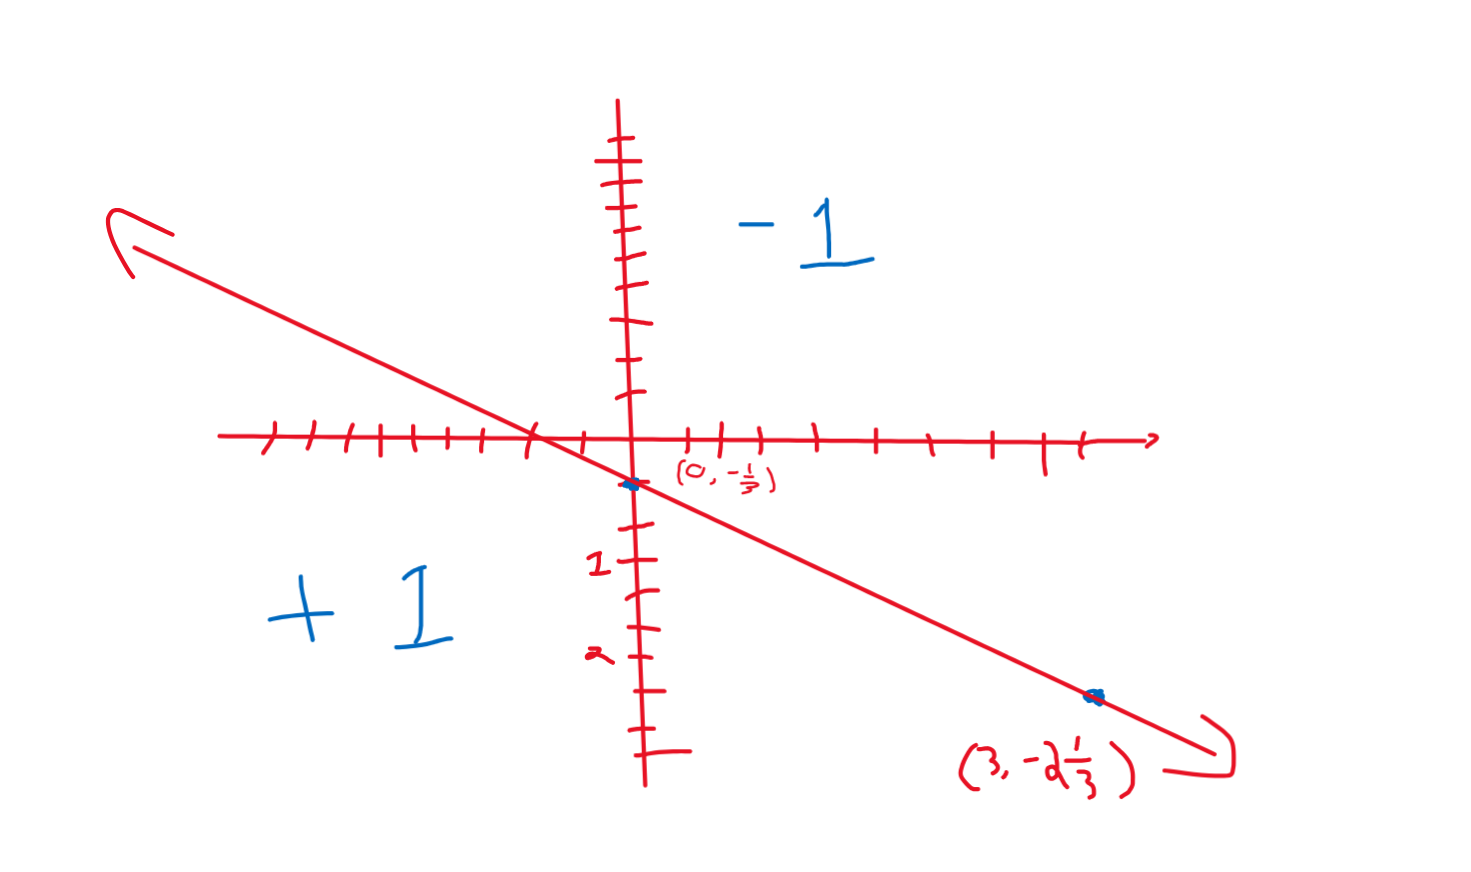
\includegraphics[width=0.6\textwidth]{negpos.png}
    \caption{Decision boundary and classification regions for $\boldsymbol{w} = -[1,2,3]^T$.}
    \label{fig:case1}
\end{figure}
}

\end{enumerate}

\item (30 points) In logistic regression (labels are \{1, -1\}),
the objective function  can be written as
$$E(w)=\frac{1}{N}\sum_{n=1}^N\ln\left(1+e^{-y_n
w^Tx_n}\right).$$ Please
\begin{enumerate}
\item (10 points) Compute the first-order derivative $\nabla E(w)$. You will
need to provide the intermediate steps of derivation.

{\color{red}

computing the gradient (deriving with respect to all variables)
\[
E(w)=\frac{1}{N}\sum_{n=1}^{N}\ln(1+e^{-y_n w^T x_n})
\]
starting with one term in the sum
\[
\ln(1+e^{-y_n w^T x_n})
\]
\[
u = -y_n w^T x_n
\]
so the expression becomes
\[
\ln(1+e^u)
\]

Using the chain rule:
\[
\frac{\partial}{\partial w}\ln(1+e^u)
=
\frac{e^u}{1+e^u}\cdot \frac{\partial u}{\partial w}
\]


\[
\frac{\partial u}{\partial w}
=
\frac{\partial}{\partial w}(-y_n w^T x_n)
=
-y_n x_n
\]

Substituting back:
\[
\frac{\partial}{\partial w}\ln(1+e^{-y_n w^T x_n})
=
\frac{e^{-y_n w^T x_n}}{1+e^{-y_n w^T x_n}}
(-y_n x_n)
\]

Simplifying the fraction  like this:
\[
\frac{e^{-z}}{1+e^{-z}} = \frac{1}{1+e^{z}}
\]

\[
=
\frac{-y_n x_n}{1+e^{y_n w^T x_n}}
\]

summing for N samples

\[
\nabla E(w)
=
-\frac{1}{N}
\sum_{n=1}^{N}
\frac{y_n x_n}{1+e^{y_n w^T x_n}}
\]
}

\item (10 points) Once the optimal $w$ is obtain, it will be used to make
predictions as follows:
\[
\mbox{Predicted class of }x =
  \begin{cases}
    1       & \quad \text{if } \theta(w^Tx)\geq 0.5\\
    -1  & \quad \text{if } \theta(w^Tx)<0.5
  \end{cases}
\]
where $\theta(z)=\frac{1}{1+e^{-z}}$.

Explain why the decision boundary of logistic regression is still
linear.

{\color{red}


\[
\theta(w^T x)=0.5
\]

using the sigmoid function
\[
\frac{1}{1+e^{-w^T x}}=0.5
\]

take the reciprocal of both sides and simplify
\[
1+e^{-w^T x}=2
\]
\[
e^{-w^T x}=1
\]
\[
-w^T x=\ln(1)
\]
\[
-w^T x=0 \implies w^T x=0
\]

Since $w^T x$ is a linear function of $x$, the decision boundary is linear.
}

\item (5 points) Is the decision boundary still linear if the prediction rule
is changed to threshold $0.9$?

{\color{red}
Yes. The boundary is defined by
\[
\theta(w^T x)=0.9
\]

\[
\frac{1}{1+e^{-w^T x}}=0.9
\]

Solving:
\[
1=0.9(1+e^{-w^T x})
\]
\[
0.1=0.9e^{-w^T x}
\]
\[
e^{-w^T x}=\frac{1}{9}
\]

natural log:
\[
-w^T x=\ln(1/9)
\]
\[
w^T x=\ln(9)
\]

this is still a linear equation of the form $w^T x = c$, it's just shifted. 
}

\item (5 points) What is the essential property that results in the
linear decision boundary?

{\color{red}
The essential property is that the input to the sigmoid function is a linear combination of the features ($w^T x$). Because the sigmoid function is monotonic, applying a threshold to the output probability is the same as applying a threshold directly to the linear input. }

\end{enumerate}

\item (10 points) Given

$$X=[x_1,x_2,\cdots,x_n]\in\mathbb{R}^{m\times n}$$
where
$x_i\in\mathbb{R}^m$ for all $i$, and
$$Y=\begin{bmatrix}
    y_1^T       \\
    y_2^T       \\
    \vdots\\
    y_n^T
\end{bmatrix}\in\mathbb{R}^{n\times p}$$
where $y_i\in\mathbb{R}^p$ for all $i$. Show that $$XY=\sum_{i=1}^n
x_i y_i^T.$$

{\color{red}

$X$ is a row vector containing $n$ columns $(x_i)$, and $Y$ is a column vector containing $n$ rows $(y_i)^T$\

Using the rule of block matrix multiplication, the product $XY$ is obtained by multiplying the corresponding rows and columns and summing them up

\begin{align*}
XY &= \begin{bmatrix} x_1 & x_2 & \cdots & x_n \end{bmatrix} \begin{bmatrix} y_1^T \\ y_2^T \\ \vdots \\ y_n^T \end{bmatrix} \\
   &= x_1 \cdot y_1^T + x_2 \cdot y_2^T + \cdots + x_n \cdot y_n^T \\
   &= \sum_{i=1}^{n} x_i y_i^T
\end{align*}

Each term $x_i y_i^T$ represents the outer product of the $i$-th column of $X$ and the $i$-th row of $Y$, giving the sum of XY
}

\item (10 points) We show that maximizing log-likelihood is
equivalent to minimizing $RSS(\boldsymbol w)$.

In particular,
$$\log\mathcal{L}(\boldsymbol{w} | \boldsymbol{x}) 
= -\frac{1}{2}\left( \frac{1}{\sigma^2}RSS(\boldsymbol{w}) + n \log \sigma^2 \right) + const$$
\begin{enumerate}
    \item (5 points) Please derive the optimal $\boldsymbol w^*$ and $\sigma^*$.
    
    {\color{red}
     To find the maximum of a function, take the derivitive with respect to the variable to care about and set it to 0. Finding $\boldsymbol{w}^*$, treat $\sigma^2$ as a constant. The terms $n \log \sigma^2$, $1/\sigma^2$, 1/2, and const become constant so we are just minimizing $RSS(\boldsymbol{w})$. Since maximizing the likely-hood would be minimizing the negative likelihood. It is giving by the normal equation:


    \textbf{1. Finding optimal $\boldsymbol{w}^*$:}
    To find $\boldsymbol{w}^*$, we treat $\sigma^2$ as a constant. The term $n \log \sigma^2$ becomes constant, so minimizing is equivalent to minimizing $RSS(\boldsymbol{w})$.
    \[
    RSS({w}) = ({y} - X{w})^T ({y} - X{w})
    \]
    Taking the gradient with respect to ${w}$ and setting it to zero:
    \[
    \nabla_{{w}} RSS({w}) = -2X^T ({y} - X{w}) = 0
    \]
    \[
    X^T X {w} = X^T {y}
    \]
      
    \[
    \boldsymbol{w}^* = (X^T X)^{-1} X^T {y}
    \]

    \textbf{2. Optimal $\sigma^*$:}
    
 $S = RSS(\boldsymbol{w}^*)$ is the sum of squared errors from our best-fit line. 

the variance of a distribution is the average squared deviation from the mean. The optimal variance is the average of the squared deviations:
\[
\sigma^2 = \frac{S}{n} = \frac{RSS(\boldsymbol{w}^*)}{n}
\]

 taking the derivative of with respect to the variance $\sigma^2$ and setting it to zero:
\[
\frac{\partial}{\partial (\sigma^2)} \left( \frac{S}{\sigma^2} + n \ln(\sigma^2) \right) = -\frac{S}{(\sigma^2)^2} + \frac{n}{\sigma^2} = 0
\]
multiplying  by $(\sigma^2)^2$:
\[
-S + n(\sigma^2) = 0 -> \sigma^2 = \frac{S}{n}
\]
\[
\sigma^* = \sqrt{\frac{RSS(\boldsymbol{w}^*)}{n}}
\]
}

    \item (5 points) What do you observe from the optimal $\sigma^*$?
    
    {\color{red}
    The optimal variance $(\sigma^*)^2$ is the \textbf{Mean Squared Error (MSE)} of the model on the training data. The best estimate for the noise variance is simply the average squared deviation of the data points from the best-fit line.
    }
\end{enumerate}

\item (10 points) Show that sigmoid function and
softmax function are the same in the binary case.
\begin{align*}
    &\mbox{sigmoid}(y) = \frac{1}{1 + e^{-y}}\\
    &\mbox{softmax}(y_j) = \frac{e^{y_j}}{\sum_{i=1}^c e^{y_i}} 
\end{align*}

{\color{red}
\textbf{Proof:}

When ($c=2$), the the class scores are $y_1$ and $y_2$. The Softmax probability for class 1 is:

\[
\text{softmax}(y_1) = \frac{e^{y_1}}{e^{y_1} + e^{y_2}}
\]

To reduce this, multiply by $e^{-y_1}$. 

\[
\text{softmax}(y_1) = \frac{e^{y_1} \cdot e^{-y_1}}{(e^{y_1} + e^{y_2}) \cdot e^{-y_1}}
\]

Denominator term 2: $e^{y_2} \cdot e^{-y_1} = e^{y_2 - y_1} = e^{-(-y_2 + y_1)} = e^{-(y_1 - y_2)}$

\[
\text{softmax}(y_1) = \frac{1}{1 + e^{-(y_1 - y_2)}}
\]

$y$ is defined as the difference between the two scores ($y = y_1 - y_2$), so plugging in y gives us:

\[
\text{softmax}(y_1) = \frac{1}{1 + e^{-y}} = \text{sigmoid}(y)
\]

Therefore, the binary case softmax function is equivalent to the sigmoid function. 
}

% \item (30 points) \textbf{Perceptron for Handwritten Digits Recognition}:
% The handwritten digits files are in the ``data'' folder: train.txt
% and test.txt. The starting code is in the ``code'' folder. In the
% data file, each row is a data example. The first entry is the digit
% label (``1'' or ``5''), and the next 256 are grayscale values
% between -1 and 1. The 256 pixels correspond to a $16\times16$ image.
% You are expected to implement your solution based on the given
% codes. The only file you need to modify is the ``solution.py'' file.
% You can test your solution by running ``main.py" file. Note that
% code is provided to compute a two-dimensional feature (symmetry and
% average intensity) from each digit image; that is, each digit image
% is represented by a two-dimensional vector before being augmented
% with a ``1'' to form a three-dimensional vector as discussed in
% class. These features along with the corresponding labels should
% serve as inputs to your Perceptron algorithm.
% {\color{red}You are expected to use Python3.}

% \begin{enumerate}
% \item (5 points) Familiarize yourself with the data by completing the \emph{show\_images} function. Include the images you plotted in your report.
% \item (5 points) In this assignment, we have already extracted two features, symmetry and
% average intensity, to distinguish between 1 and 5. Familiarize
% yourself with the features by completing the \emph{show\_features}
% function and include the 2-D scatter plot into your report. For each
% sample, plot the two features with a red \textcolor{red}{$*$} if the
% label is 1 and a blue \textcolor{blue}{$+$}  if the label is 5.
% \item (10 points) Complete the \emph{Perceptron} class. You can test your
% accuracy results using the ``test_accuracy'' function in
% ``main.py''.
% \item (10 points) Complete the \emph{show\_result} function to plot the
% test data with the separators. Include the images you plotted into
% your report.
% \end{enumerate}

% \textbf{Deliverable:} You should submit (1) a report
% (along with your write-up for other questions) that summarizes your
% results and (2) the ``solution.py'' file to the Canvas.

% \textbf{Note:} Please read the ``Readme.txt'' file carefully before
% you start this assignment. Please do {\color{red} NOT} change anything in the
% ``main.py'' and ``helper.py'' files when you program.

\end{enumerate}



\end{document}